%\documentclass[a4paper]{article}
%\usepackage[utf8]{inputenc}
\usepackage[spanish, es-tabla, es-noshorthands]{babel}
\usepackage[table,xcdraw,dvipsnames]{xcolor}
\usepackage[a4paper, footnotesep=1.25cm, headheight=1.25cm, top=2.54cm, left=2.54cm,
 bottom=2.54cm, right=2.54cm]{geometry}
%\geometry{showframe}
 \usepackage[normalem]{ulem}
 \useunder{\uline}{\ul}{}

%VERIFICAR EL HEAD Y EL FOOT EN
%https://ctan.dcc.uchile.cl/macros/latex/contrib/geometry/geometry.pdf

%Paquetes varios:
\usepackage{verbatimbox}

%\usepackage{wrapfig}			%Wrap figure in text
\usepackage[export]{adjustbox}	%Move images
\usepackage{changepage}			%Move tables
\usepackage{todonotes}

\usepackage{tikz}
\usepackage{amsmath}
\usepackage{amsfonts}
\usepackage{amssymb}
\usepackage{float}
\usepackage[graphicx]{realboxes}
\usepackage{caption}
\usepackage{subcaption}
\usepackage{multicol}
\usepackage{multirow}
\setlength{\doublerulesep}{\arrayrulewidth}
%\usepackage{booktabs}

\usepackage{array}
\newcolumntype{C}[1]{>{\centering\let\newline\\\arraybackslash\hspace{0pt}}m{#1}}
%\usepackage[american]{circuitikz}
\usetikzlibrary{calc}
\usepackage{fancyhdr}
\usepackage{units} 

\usepackage{colortbl}
%\usepackage{sectsty}
%\usepackage{unicode-math}

%FONTS (IMPORTANTE): Compilar en XeLaTex o LuaLaTeX
\usepackage{anyfontsize}	%Font size
\usepackage{fontspec}		%Font type
%Si sigue sin andar comentar \usepackage[utf8]{inputenc}
%https://ctan.dcc.uchile.cl/macros/unicodetex/latex/fontspec/fontspec.pdf
%https://www.overleaf.com/learn/latex/XeLaTeX

%Path para imagenes para trabajar en subarchivos
\graphicspath{{../Resumen/}{../Referencias/}{../Apendice/}{../Descripción de la Empresa/}{../Tareas del Alumno/}{../Conclusiones/}{../Herramientas Empleadas/}}

%Definiciones de nuevos comandos y colores
%COLORES:
\definecolor{AzulFoot}{rgb}{0.682,0.809,0.926}	%RGB	%{174,206,235}
\definecolor{AzulInfo}{rgb}{0.180,0.455,0.710}	%RGB	%{46,116,181}
\definecolor{AzulTable}{rgb}{0.302,0.507,0.871}	%RGB	%{68,114,196}
\definecolor{PName}{rgb}{0.353,0.353,0.353}		%RGB	%{90,90,90}
\definecolor{mygreen}{rgb}{28,172,0} % color values Red, Green, Blue
\definecolor{mylilas}{rgb}{170,55,241}

%Change Font Size

% #1 = size, #2 = text
\newcommand{\setparagraphsize}[2]{{\fontsize{#1}{6}\selectfont#2 \par}}		%Cambia el size de todo el parrafo
\newcommand{\setlinesize}[2]{{\fontsize{#1}{6}\selectfont#2}}				%Cambia el font de una oración

%IMAGE IN TABLE:			%Ejemplo: \includeintable{.3}{ImagenesFactibilidad/pend}
\renewcommand\fbox{\fcolorbox{white}{white}}
\setlength{\fboxrule}{0pt}	%padding thickness
\setlength{\fboxsep}{4pt}	%border thickness
\newcommand{\includeintable}[2]{	
	\fbox{
		\begin{minipage}{#1\textwidth}
        	\includegraphics[width=\linewidth]{#2}
    	\end{minipage}
	}
}

%LINK IN REF
\newcommand{\reflink}[1]{		%LINK
	\href{#1}{#1}
}

%NOTAS:
\newcommand{\note}[1]{		%RED BIG NOTE (TODO)
	\begin{center}
		\huge{ \textcolor{red}{#1} }
	\end{center}
}

\newcommand{\lnote}[1]{{\fontsize{14}{6}\selectfont\textcolor{green}{#1}}}	%Notas pequeñas

\newcommand{\observacion}[2]{  \ifnumequal{1}{#1}{ { \todo[inline,backgroundcolor=red!25,bordercolor=red!100]{\textbf{Observación: #2}} } }{  }  }

\newcommand{\red}[1]{\textcolor{red}{#1}}

\newcommand{\TBD}{\textcolor{red}{(TBD) }}
\newcommand{\tbd}{\textcolor{red}{(TBD) }}

\newcommand{\TBC}{\textcolor{red}{(TBC) }}
\newcommand{\tbc}{\textcolor{red}{(TBC) }}

\newcommand{\quotes}[1]{``#1''}
\newcommand{\q}[1]{``#1''}

\newcommand{\ip}{192.168.0.10:1880}
\newcommand{\ipadmin}{192.168.0.10:1880/admin}

% Comandos para agregar elementos en tablas de acronimos y definiciones
\newcommand{\addacronym}[2]{\textbf{#1} & \begin{tabular}[l]{@{}l@{}}#2\end{tabular} \\ \hline}

% tabItem
\newcommand{\tabitem}{~~\llap{\textbullet}~~}


\usepackage{hyperref}
\hypersetup{
    colorlinks=true,
    linkcolor=black,
    filecolor=magenta,      
    urlcolor=AzulInfo,
    citecolor=AzulInfo,    
}

%Configuración del header y del footer:
\usepackage{etoolbox}
\pagestyle{fancy}
\fancyhf{}
\rfoot{\thepage}
\renewcommand{\footrulewidth}{4pt}
\renewcommand{\headrulewidth}{0pt}
\patchcmd{\footrule}{\hrule}{\color{AzulFoot}\hrule}{}{}

%Código en el informe
%% IMPORTANTE:
% Verificar que esté \usepackage[dvipsnames]{xcolor}

%\usepackage{listingsutf8}
\usepackage{listings}

\renewcommand{\lstlistingname}{Código}

%LSTSET: Pone un recuadro y contador de linea en el codigo
\newcommand{\boxstyle}{
	\lstset{
		basicstyle=\sffamily\color{black},
		frame=single,
		numbers=left,
		numbersep=5pt,
		numberstyle=\color{gray},
		showspaces=false,
		showstringspaces=false
	}
}

\newcommand{\defaultstyle}{
	\lstset{
		basicstyle=\sffamily\color{white},
		frame=none,
		numbers=none,
		showspaces=true,
		showstringspaces=true
	}
}

\lstdefinelanguage{Kotlin}{
  captionpos=b,
  comment=[l]{//},
  commentstyle={\color{gray}\ttfamily},
  emph={filter, first, firstOrNull, forEach, lazy, map, mapNotNull, println},
  emphstyle={\color{OrangeRed}},
  identifierstyle=\color{black},
  keywords={!in, !is, abstract, actual, annotation, as, as?, break, by, catch, class, companion, const, constructor, continue, crossinline, data, delegate, do, dynamic, else, enum, expect, external, false, field, file, final, finally, for, fun, get, if, import, in, infix, init, inline, inner, interface, internal, is, lateinit, noinline, null, object, open, operator, out, override, package, param, private, property, protected, public, receiveris, reified, return, return@, sealed, set, setparam, super, suspend, tailrec, this, throw, true, try, typealias, typeof, val, var, vararg, when, where, while},
  keywordstyle={\color{NavyBlue}\bfseries},
  morecomment=[s]{/*}{*/},
  morestring=[b]",
  morestring=[s]{"""*}{*"""},
  ndkeywords={@Deprecated, @JvmField, @JvmName, @JvmOverloads, @JvmStatic, @JvmSynthetic, Array, Byte, Double, Float, Int, Integer, Iterable, Long, Runnable, Short, String, Any, Unit, Nothing},
  ndkeywordstyle={\color{BurntOrange}\bfseries},
  sensitive=true,
  stringstyle={\color{ForestGreen}\ttfamily},
}

\lstdefinelanguage{Swift}
{
  morekeywords={
    open,catch,@escaping,nil,throws,func,if,then,else,for,in,while,do,switch,case,default,where,break,continue,fallthrough,return,
    typealias,struct,class,enum,protocol,var,func,let,get,set,willSet,didSet,inout,init,deinit,extension,
    subscript,prefix,operator,infix,postfix,precedence,associativity,left,right,none,convenience,dynamic,
    final,lazy,mutating,nonmutating,optional,override,required,static,unowned,safe,weak,internal,
    private,public,is,as,self,unsafe,dynamicType,true,false,nil,Type,Protocol,
  },
  morecomment=[l]{//}, % l is for line comment
  morecomment=[s]{/*}{*/}, % s is for start and end delimiter
  morestring=[b]", % defines that strings are enclosed in double quotes
  breaklines=true,
  escapeinside={\%*}{*)},
  numbers=left,
  captionpos=b,
  breakatwhitespace=true,
  basicstyle=\linespread{1.0}\ttfamily, % https://tex.stackexchange.com/a/102728/129441
}

\definecolor{keyword}{HTML}{BA2CA3}
\definecolor{string}{HTML}{D12F1B}
\definecolor{comment}{HTML}{008400}

\newcommand{\swiftstyle}{
	\lstset{
  		language=Swift,
  		inputencoding=utf8x,
		extendedchars=\true,
	  	basicstyle=\ttfamily,
	  	showstringspaces=false, % lets spaces in strings appear as real spaces
  		columns=fixed,
  		keepspaces=true,
  		keywordstyle=\color{keyword},
  		stringstyle=\color{string},
  		commentstyle=\color{comment}
	}
}


%Como usarlo:

%\begin{lstlisting}[caption={Simple code listing.}, label={lst:example1}, language=Kotlin]
%// this is a simple code listing:
%println("hello kotlin from latex")
%\end{lstlisting}

%Si se corta en 2 páginas distintas:

%\vspace{1mm}
%\noindent{\begin{minipage}{\linewidth}
%\begin{lstlisting}[...]
%...
%\end{lstlisting}
%\end{minipage}}




\usepackage{titlesec}		%Para hacer las subsubsubsections

%Colores a los nombres de las secciones:
%\sectionfont{\color{AzulInfo}}  % sets color of sections
%\subsectionfont{\color{AzulInfo}}
%\subsubsectionfont{\color{AzulInfo}}

%PICTURES AND TABLE INDEX:
\newcommand{\Section}[1]{ \section{#1} 
	\phantomsection \setcounter{figure}{0} \setcounter{table}{0} \setcounter{lstlisting}{0}
		\renewcommand{\thetable}{\arabic{section}.\arabic{table}}
		\renewcommand{\thefigure}{\arabic{section}.\arabic{figure}}
		\renewcommand{\thelstlisting}{\arabic{section}.\arabic{lstlisting}}
}

\newcommand{\Subsection}[1]{ \subsection{#1}
	\phantomsection \setcounter{figure}{0} \setcounter{table}{0} \setcounter{lstlisting}{0}
		\renewcommand{\thetable}{\arabic{section}.\arabic{subsection}.\arabic{table}}
		\renewcommand{\thefigure}{\arabic{section}.\arabic{subsection}.\arabic{figure}}
		\renewcommand{\thelstlisting}{\arabic{section}.\arabic{subsection}.\arabic{lstlisting}}
}

\newcommand{\Subsubsection}[1]{ \subsubsection{#1} 
	\phantomsection \setcounter{figure}{0} \setcounter{table}{0}  \setcounter{lstlisting}{0}
		\renewcommand{\thetable}{\arabic{section}.\arabic{subsection}.\arabic{subsubsection}.\arabic{table}}
		\renewcommand{\thefigure}{\arabic{section}.\arabic{subsection}.\arabic{subsubsection}.\arabic{figure}}
		\renewcommand{\thelstlisting}{\arabic{section}.\arabic{subsection}.\arabic{subsubsection}.\arabic{lstlisting}}
}

%Definición de subsubsubsection:
\titleclass{\subsubsubsection}{straight}[\subsection]

\newcounter{subsubsubsection}[subsubsection]
\renewcommand\thesubsubsubsection{\thesubsubsection.\arabic{subsubsubsection}}

\titleformat{\subsubsubsection}
  {\normalfont\normalsize\bfseries\color{AzulInfo}}{\thesubsubsubsection}{1em}{}	%Color de subsubsubsection
\titlespacing*{\subsubsubsection}
{0pt}{3.25ex plus 1ex minus .2ex}{1.5ex plus .2ex}

\makeatletter
\renewcommand\paragraph{\@startsection{paragraph}{5}{\z@}%
  {3.25ex \@plus1ex \@minus.2ex}%
  {-1em}%
  {\normalfont\normalsize\bfseries}}
\renewcommand\subparagraph{\@startsection{subparagraph}{6}{\parindent}%
  {3.25ex \@plus1ex \@minus .2ex}%
  {-1em}%
  {\normalfont\normalsize\bfseries}}
\def\toclevel@subsubsubsection{4}
\def\toclevel@paragraph{5}
\def\toclevel@paragraph{6}
\def\l@subsubsubsection{\@dottedtocline{4}{7em}{4em}}
\def\l@paragraph{\@dottedtocline{5}{10em}{5em}}
\def\l@subparagraph{\@dottedtocline{6}{14em}{6em}}
\makeatother

\setcounter{secnumdepth}{4}
\setcounter{tocdepth}{4}

%Subsubsubsection:
\newcommand{\Subsubsubsection}[1]{ \subsubsubsection{#1} 
	\phantomsection \setcounter{figure}{0} \setcounter{table}{0} \renewcommand{\thetable}{\arabic{section}.\arabic{subsection}.\arabic{subsubsection}.\arabic{subsubsubsection}.\arabic{table}} \renewcommand{\thefigure}{\arabic{section}.\arabic{subsection}.\arabic{subsubsection}.\arabic{subsubsubsection}.\arabic{figure}}
}

%Tamaño, color e identación de sección, subsección, subsubsección y subsubsubsección:
%La identación de las subsecciones está tambien en Index-cfg.tex para el toc, lot y lot en el index
\titleformat{\section}[block]{\fontsize{16}{6}\selectfont\bfseries\color{AzulInfo}}{\thesection.}{1em}{} 
\titleformat{\subsection}[block]{\hspace{2.5em}\fontsize{13}{6}\selectfont\color{AzulInfo}}{\thesubsection}{1em}{}
\titleformat{\subsubsection}[block]{\hspace{3.5em}\fontsize{12}{6}\selectfont\color{AzulInfo}}{\thesubsubsection}{1em}{}
\titleformat{\subsubsubsection}[block]{\hspace{4em}\fontsize{11}{6}\selectfont\color{AzulInfo}}{\thesubsubsubsection}{1em}{}

%Pone las refrencias en el indice
\usepackage[numbib, nottoc, notlot, notlof]{tocbibind}

%Pone toc, lof y lot en colores y elijo el titulo de estos
\addto\captionsspanish{
	\renewcommand\contentsname{Contenidos}
	\renewcommand\listfigurename{Lista de Figuras}
	\renewcommand\listtablename{Lista de Tablas}
}

%Agrega TOC al indice
\renewcommand{\tableofcontents}{
	\stepcounter{section}
	\addcontentsline{toc}{section}{\protect\numberline{\thesection}\textbf{Contenidos}}
	\tableofcontents
}

%Agrega LOF al indice
\renewcommand{\listoffigures}{
	\stepcounter{section}
	\addcontentsline{toc}{section}{\protect\numberline{\thesection}\textbf{Lista de Figuras}}
	\listoffigures
}

%Agrega LOT al indice
\renewcommand{\listoftables}{
	\stepcounter{section}
	\addcontentsline{toc}{section}{\protect\numberline{\thesection}\textbf{Lista de Tablas}}
	\listoftables
}

%Indices: cambio la separación de los numeros para que entren tablas y fotos
\usepackage{tocloft}
\setlength{\cftfignumwidth}{1.35cm}  % change numwidth from figures in lof
\setlength{\cfttabnumwidth}{1.35cm}  % change numwidth from tables in lot
\renewcommand{\cfttoctitlefont}{\Large\bfseries\color{AzulInfo}}
\renewcommand{\cftloftitlefont}{\Large\bfseries\color{AzulInfo}}
\renewcommand{\cftlottitlefont}{\Large\bfseries\color{AzulInfo}}

%Coloca lineas punteadas a las seciones en el TOC
\renewcommand{\cftsecleader}{\cftdotfill{\cftdotsep}}

%Items con bullets y no cuadrados
\renewcommand{\labelitemi}{\textbullet }

%
%\begin{document}

\Subsection{Hardware}

\Subsubsection{Diagrama de bloques (Hardware)}
A continuaci\'on se muestra el diagram en bloques del Hardware y los delimitadores de las secciones, siendo estas:
\begin{itemize}
\item Potencia
\item Cargador
\item Sensado
\end{itemize}

\begin{figure}[H]
	\centering
	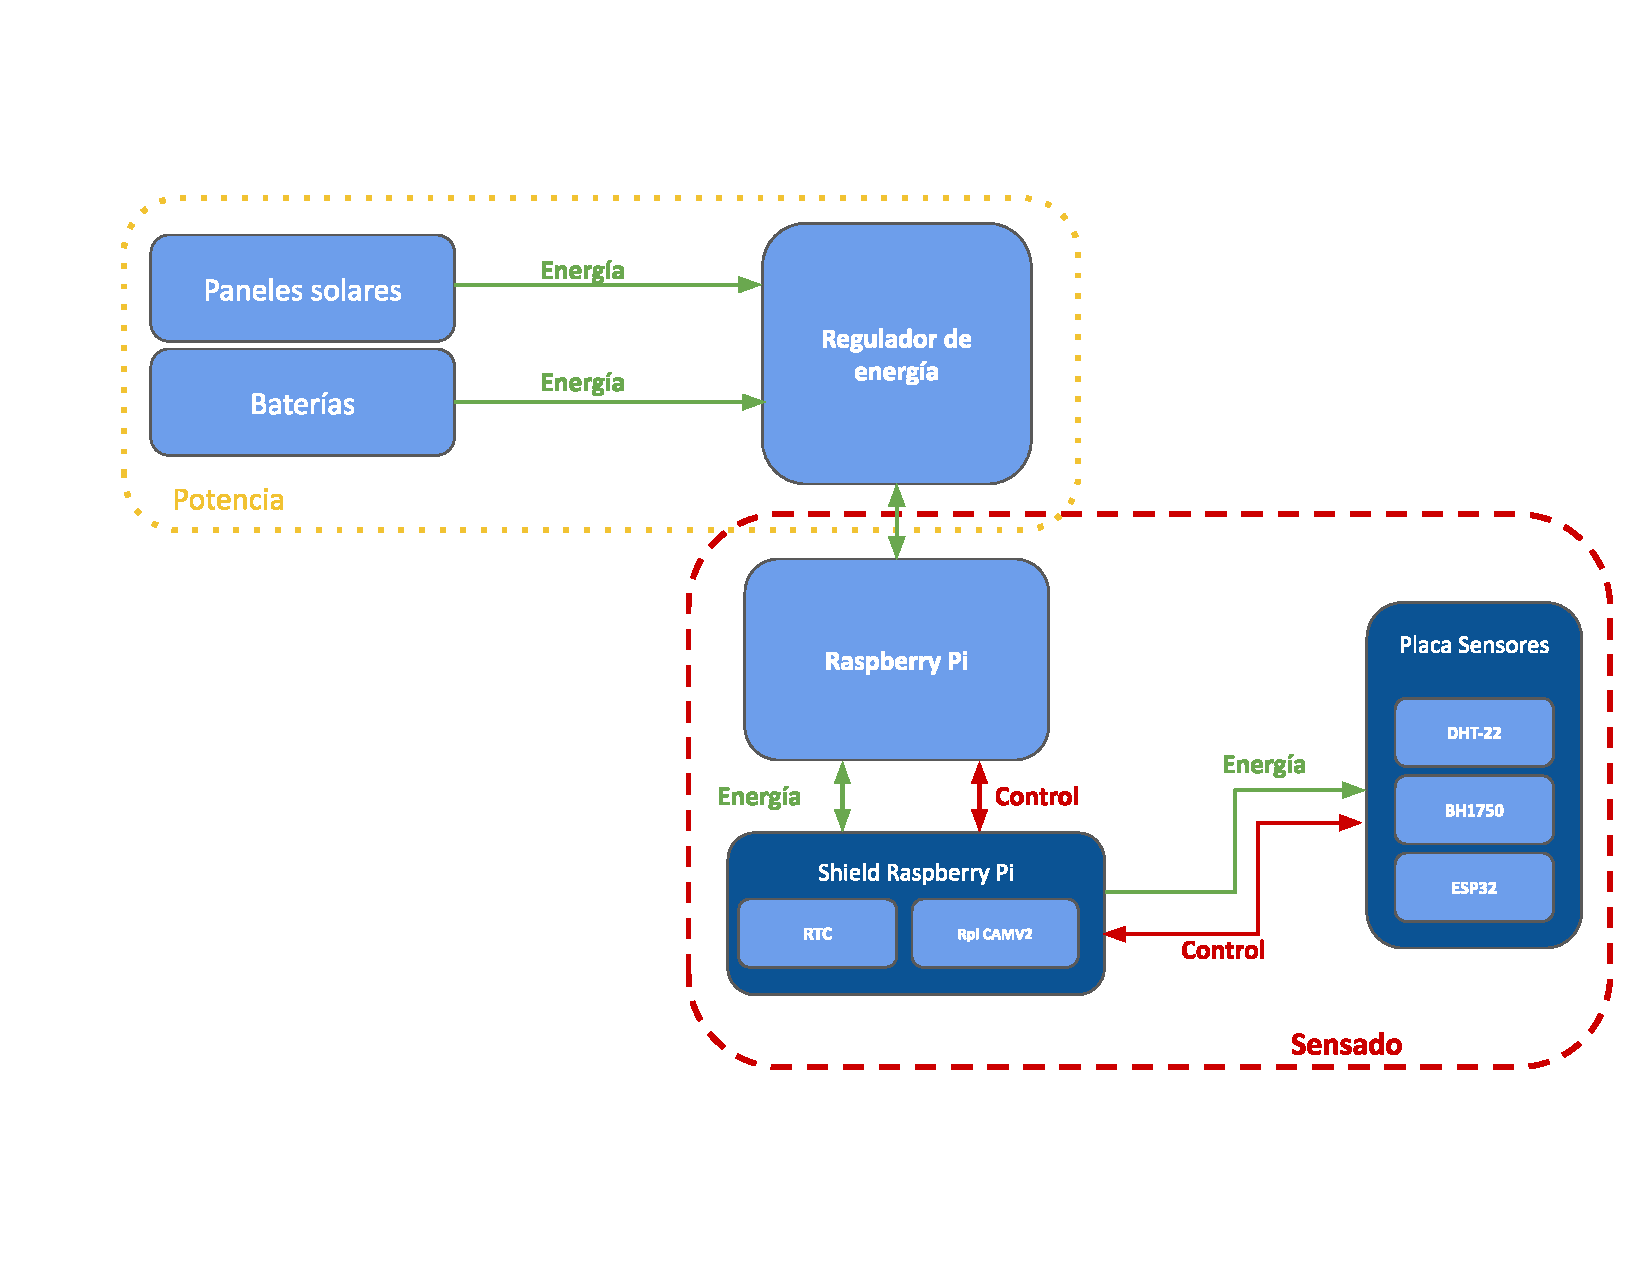
\includegraphics[width=0.7\linewidth]{ImagenesIngenieria de Detalle/DiagramaHardwareMarcado}
	\label{fig:diagrama_hardware}
	\caption{Diagrama en bloques del sistema de hardware.}
\end{figure}
La etapa de potencia es el conjunto de elementos necesarios para proveer de energ\'ia a toda la electr\'onica del proyecto.

El cargador es la etapa que se encarga, como su nombre indica realizar al carga inal\'ambrica de la UBM.

Y la de sensado se encarga de la medici\'on de las variables f\'isicas y de su correcto almacenamiento, teniendo en cuenta que esto implica un conocimiento preciso de la hora.



\Subsubsection{Descripción detallada de cada bloque}
\input{../Ingenieria de Detalle/Hardware/Descripción detallada de cada bloque.tex}

\Subsubsection{Detalles de selección y cálculo de los elementos circuitales de cada bloque}
\input{../Ingenieria de Detalle/Hardware/Detalles de selección.tex}

\Subsubsection{Plan de pruebas de cada modulo}
El plan de pruebas corresponde a las descritas en [\ref{sec:BancoDePruebas}].
Para el uso correcto de los módulos se tuvieron en cuenta los siguientes aspectos:
\begin{itemize}
	\item Definir un estado predeterminado del Bus $I^2C$ mediante \textit{pullups}.
	\item El uso de capacitores de desacople
	\item Para el módulo RTC, el integrado DS1307 requiere $5 \ V$ para funcionar correctamente, por lo que para que sea compatible con la lógica de $3.3 \ V$ de la \rspi, se realiza un cambio en el esquemático al remover dos resistores del módulo.
\end{itemize}

\begin{figure}[H]
	\centering
	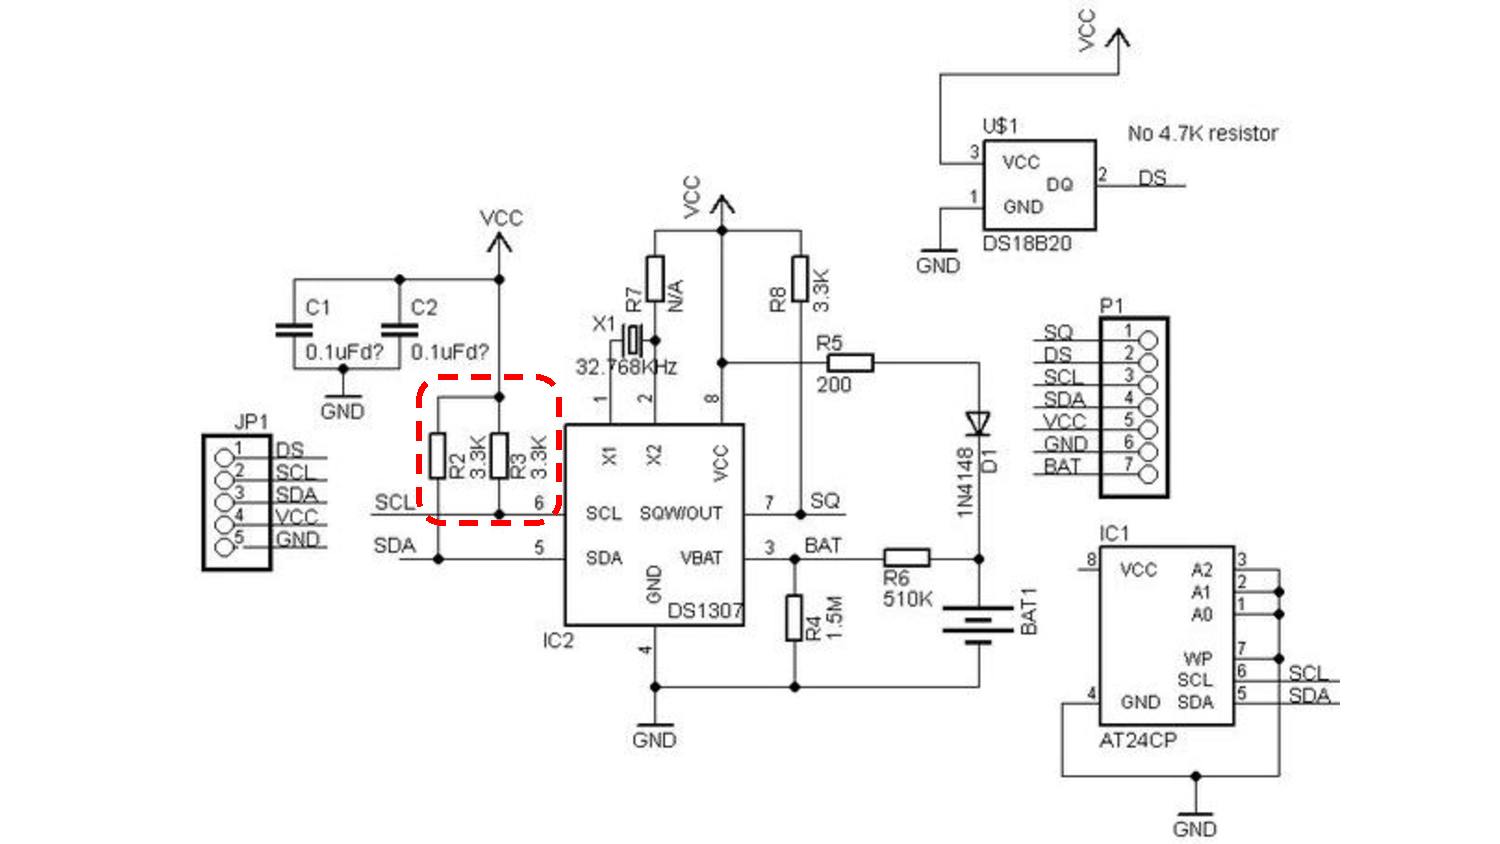
\includegraphics[width=0.9\linewidth,page=1]{ImagenesIngenieria de detalle/rtcTinySchematic}
	\caption{Esquemático RTC-Tiny.}
	\label{fig:RTCSchematic}
\end{figure}

Con este cambio se quita la referencia a $5 \ V$ del bus en el módulo. Por lo que la lógica queda en el rango de $3.3 \ V$ a $5 \ V$. Cabe destacar que utilizar los niveles lógicos de $3.3 \ V$ son compatibles con el integrado $DS1307$




\Subsection{Software}

\Subsubsection{Esquema general del proyecto}
\note{Mi idea para esta parte era explicar que tecnologías íbamos a usar y eso}

\Subsubsection{Diagrama de estados y flujogramas}
En este pasaje se muestran los diagramas de estados del sistema. Es así que se puede notar que el conjunto cuenta con 4 estados distintivos, siendo estos los llamados \textit{Initial}, \textit{Idle}, \textit{Charging} y \textit{Communicating}.

Vale la pena mencionar que en cualquiera de los estados, a excepción de \textit{Initial}, el sistema esta realizando mediciones del ambiente mientras cuenta también con la posibilidad de comunicarse por Bluetooth con la electrónica de la mochila. Esto se cumple excluyendo el caso en que el nivel de carga de la UBM no sea suficiente.

\begin{figure}[H]
	\centering
	%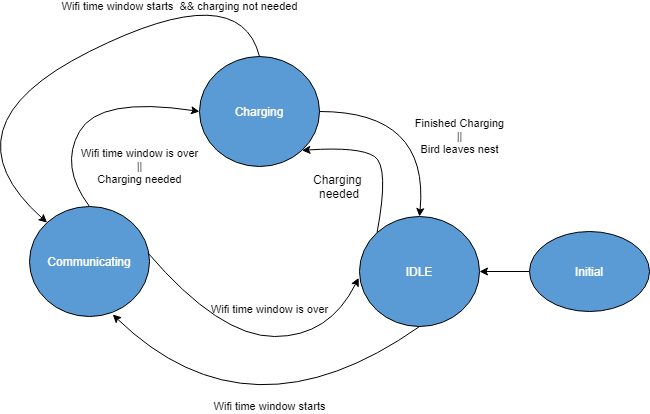
\includegraphics[width=0.9\linewidth]{ImagenesIngenieria de Detalle/Diagrama_de_Estados}	
	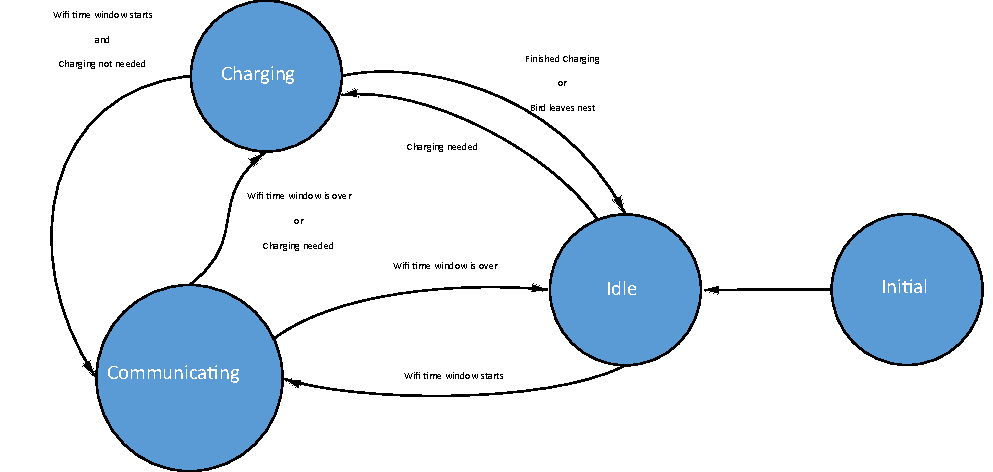
\includegraphics[width=\textwidth, page=1]{ImagenesIngenieria de Detalle/FlowChart.pdf}	
	\caption{Diagrama de estados.}
	\label{fig:Diagrama_de_Estados}
\end{figure}

En el estado \textit{Initial} es aquel donde se inicializan todos los drivers, estructuras de datos y configuraciones que se encuentren por defecto. No se vuelve a este estado una vez que este haya sido abandonado. 

\begin{figure}[H]
	\centering
	%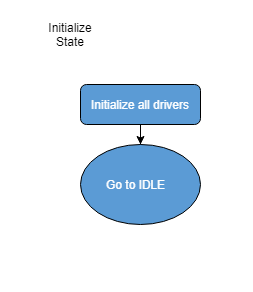
\includegraphics[width=0.4\linewidth]{ImagenesIngenieria de Detalle/diagrama_flujo_initial}	
	\includegraphics[width=0.2\textwidth, page=5]{ImagenesIngenieria de Detalle/FlowChart.pdf}	
	\caption{Diagrama de flujo: Estado Initial.}
	\label{fig:Diagrama_de_flujo_init}
\end{figure}

Luego se encuentra el estado \textit{Idle}. En este se sensan las variables físicas con el periodo de muestreo acorde a la especificaciones 10, 11, 12 y 13 de la Tabla (\ref{tab:intFun}). Luego se fija si es momento de prender el hotspot wifi. En caso afirmativo se irá al estado \textit{Communicating}. En caso contrario se analiza si hay que cargar la batería. Si se debe realizar dicha acción se irá a estado \textit{Charging}, minetras que en el caso opuesto, si hay transmisión Bluetooth, actua acorde y comienza el ciclo nuevamente.

\begin{figure}[H]
	\centering
	%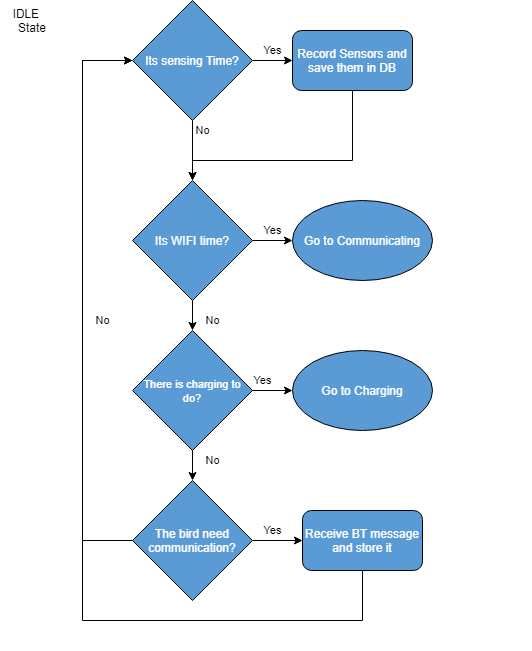
\includegraphics[width=0.9\linewidth]{ImagenesIngenieria de Detalle/diagrama_flujo_idle}	
	\includegraphics[width=0.6\textwidth, page=4]{ImagenesIngenieria de Detalle/FlowChart.pdf}	
	\caption{Diagrama de flujo: Estado \textit{Iddle}.}
	\label{fig:Diagrama_de_flujo_idle}
\end{figure}

La función principal del estado \textit{Charging} es la de cargar la UBM. Lo primero se hace en este estado es habilitar el cargador, luego, en caso de que haya un mensaje Bluetooth, se comienza la comunicación. Posteriormente se encarga del sensado, se verifica si la carga se terminó, para que cuando esto ocurra se desactive el cargador. Dependiendo si es momento de habilitar el hotspot o no se irá al estado \textit{Communicating} o \textit{Idle}.

\begin{figure}[H]
	\centering
	%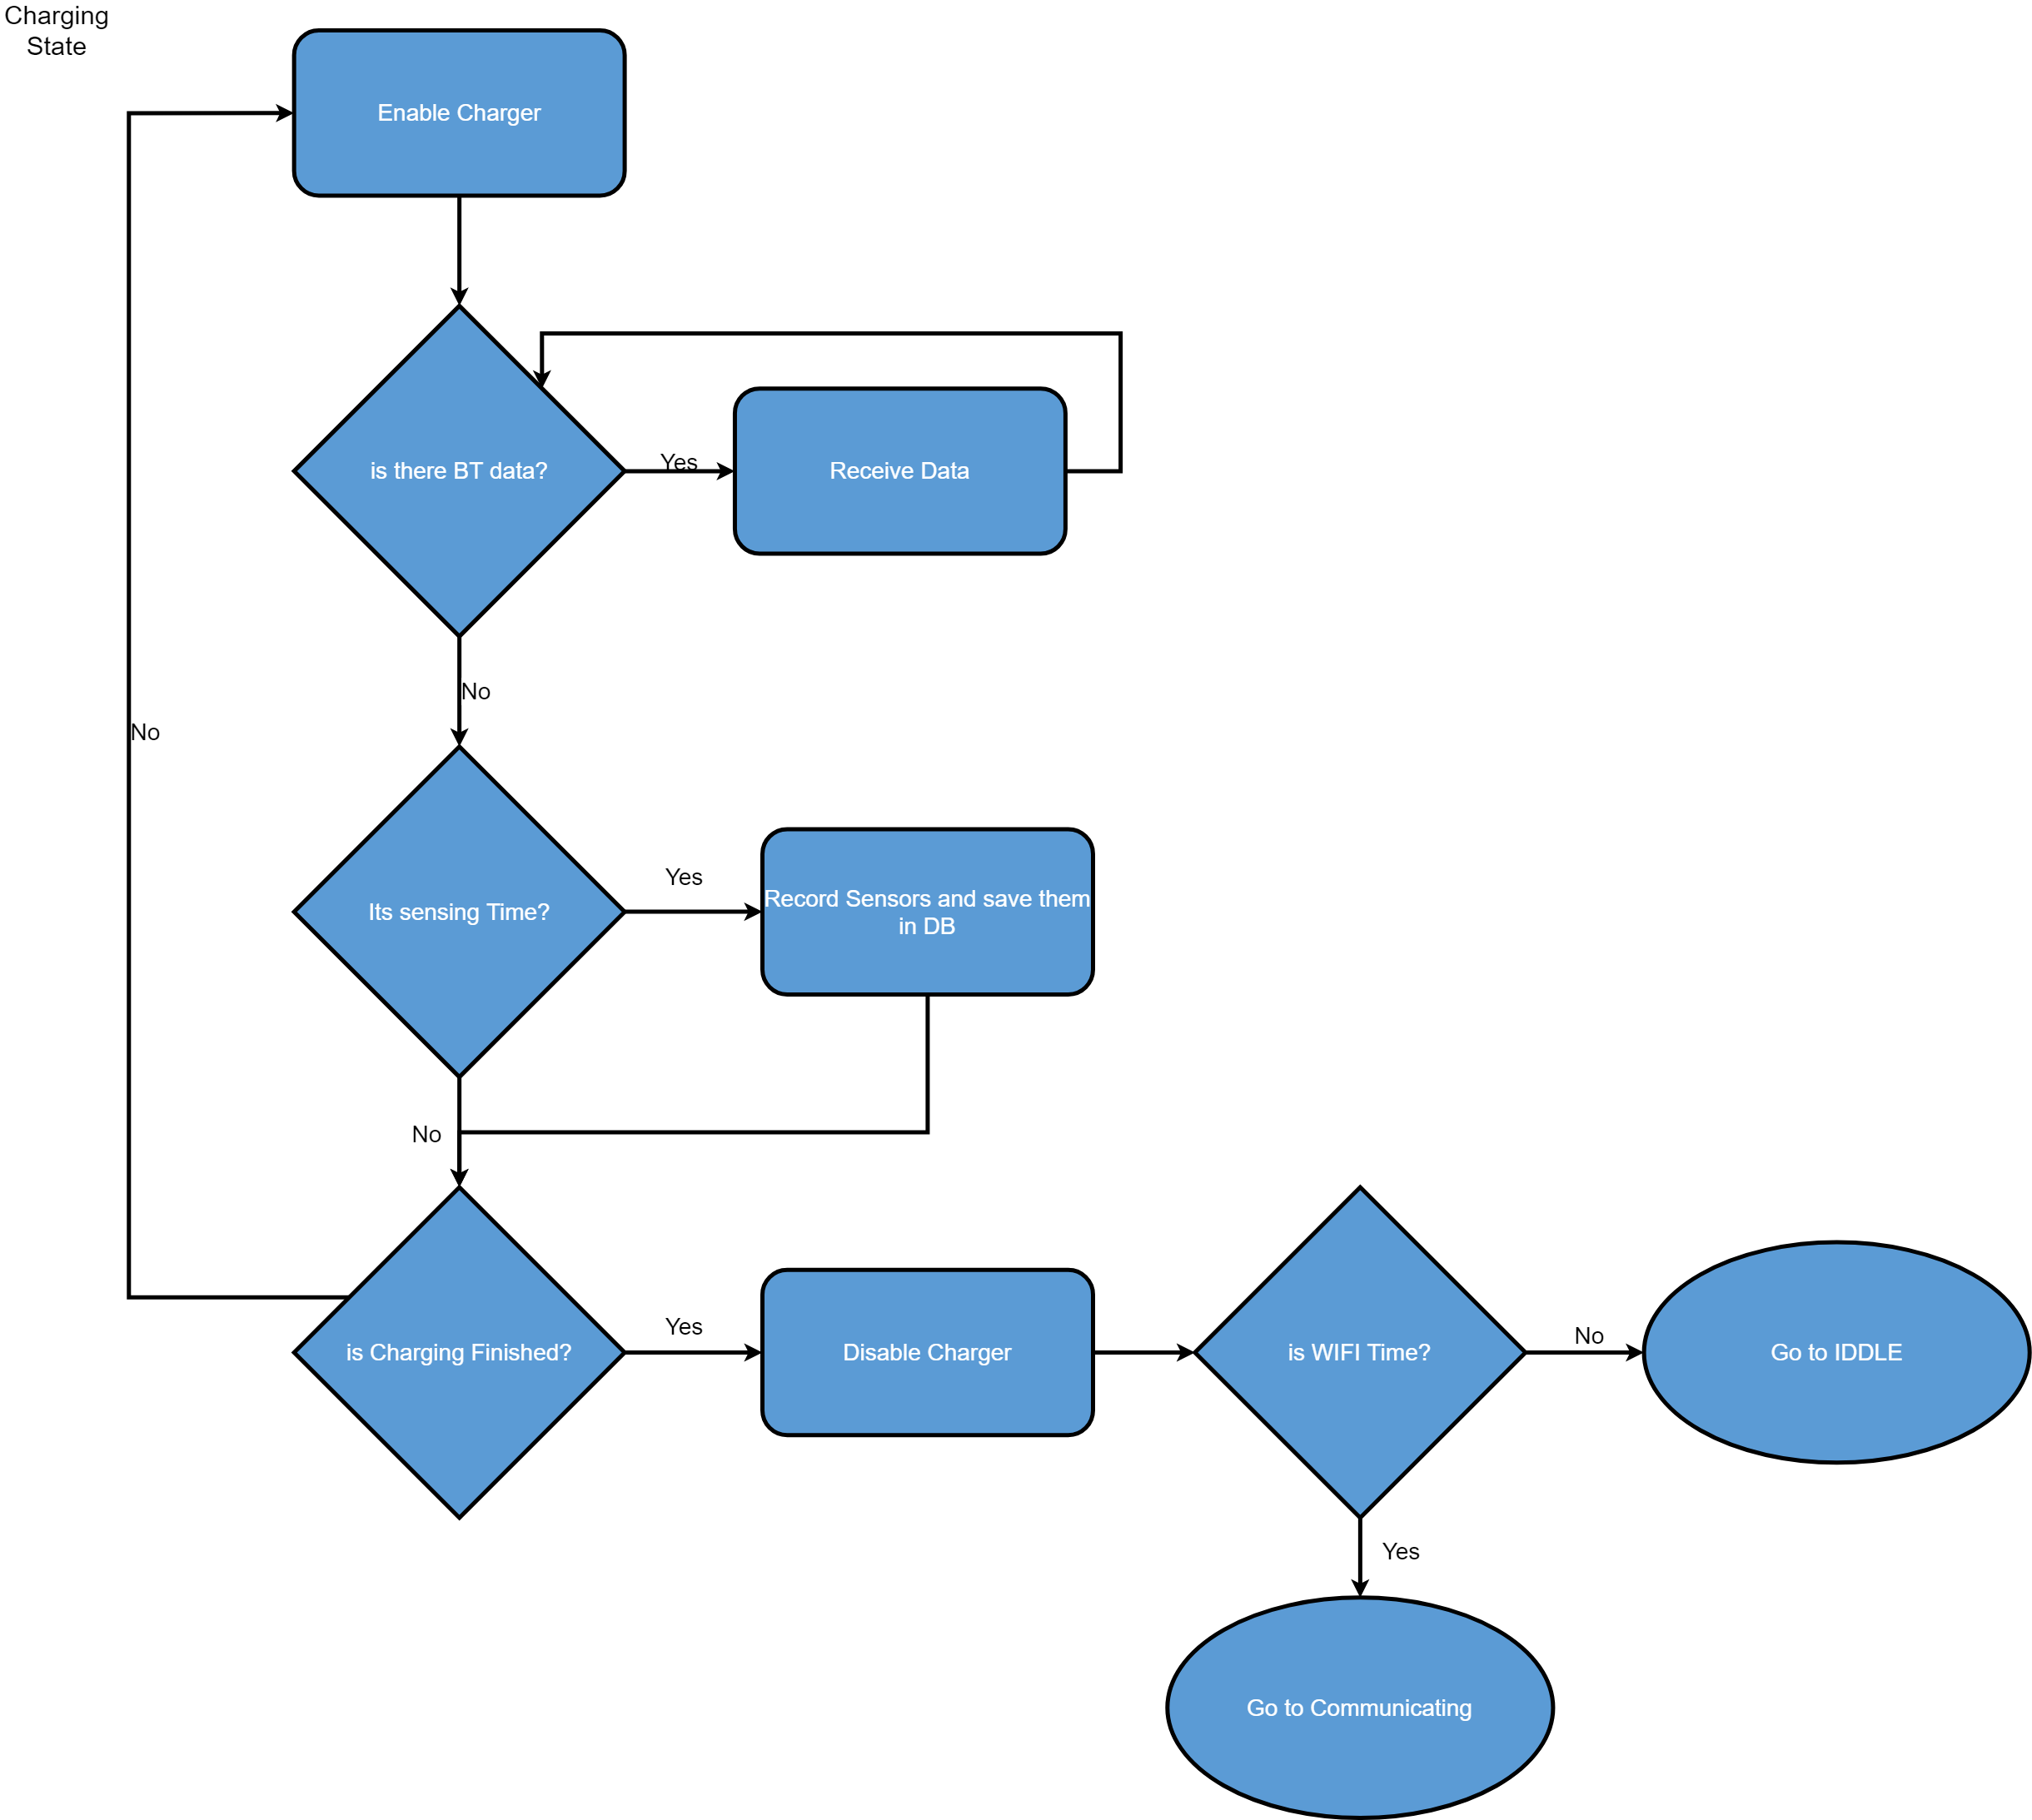
\includegraphics[width=0.9\linewidth]{ImagenesIngenieria de Detalle/diagrama_flujo_charging}	
	\includegraphics[width=0.7\textwidth, page=2]{ImagenesIngenieria de Detalle/FlowChart.pdf}
	\caption{Diagrama de flujo: Estado \textit{Charging}.}
	\label{fig:Diagrama_de_flujo_charging}
\end{figure}

Finalmente en el estado \textit{Communicating} es aquel en el que se habilita el hotspot y se levanta el servidor de Node-Red. Aquí se realiza la comunicación entre el nido y una computadora en al base del árbol. Esto se mantendrá hasta que haya pasado el tiempo especificado en \lnote{En el esquema general de software habria que especificarlo O en especificaciones}. Además, se continua sensando las variables físicas.

\begin{figure}[H]
	\centering
	%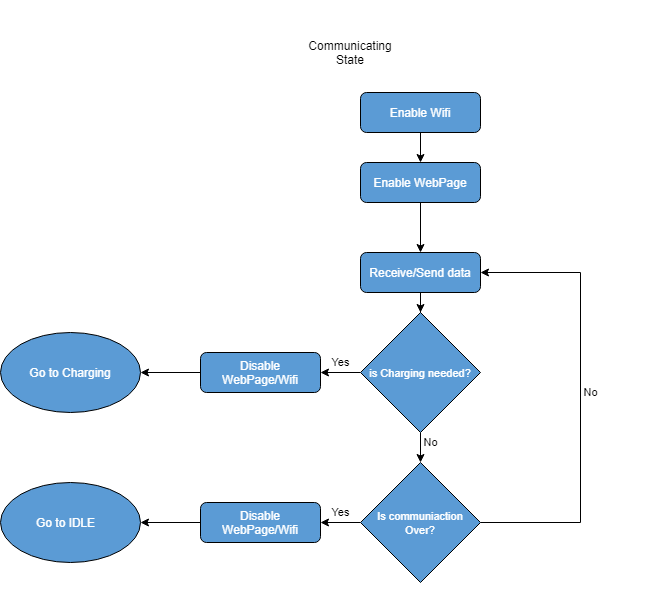
\includegraphics[width=0.9\linewidth]{ImagenesIngenieria de Detalle/diagrama_flujo_communicating}	
	\includegraphics[width=0.9\textwidth, page=3]{ImagenesIngenieria de Detalle/FlowChart.pdf}
	\caption{Diagrama de flujo: Estado \textit{Communicating}.}
	\label{fig:diagrama_flujo_communicating}
\end{figure}

\Subsubsection{Análisis de complejidad}
\input{../Ingenieria de Detalle/Software/Análisis de complejidad.tex}

\Subsubsection{Descripción de subrutinas}
\input{../Ingenieria de Detalle/Software/Descripción de subrutinas.tex}

\Subsubsection{Listado de elementos del código}
\TBD

\Subsubsection{Plan de prueba de módulos y de depuración de Software}
El plan de pruebas corresponde a las descritas en [\ref{sec:BancoDePruebas}].
Para el uso correcto de los módulos se tuvieron en cuenta los siguientes aspectos:
\begin{itemize}
	\item Definir un estado predeterminado del Bus $I^2C$ mediante \textit{pullups}.
	\item El uso de capacitores de desacople
	\item Para el módulo RTC, el integrado DS1307 requiere $5 \ V$ para funcionar correctamente, por lo que para que sea compatible con la lógica de $3.3 \ V$ de la \rspi, se realiza un cambio en el esquemático al remover dos resistores del módulo.
\end{itemize}

\begin{figure}[H]
	\centering
	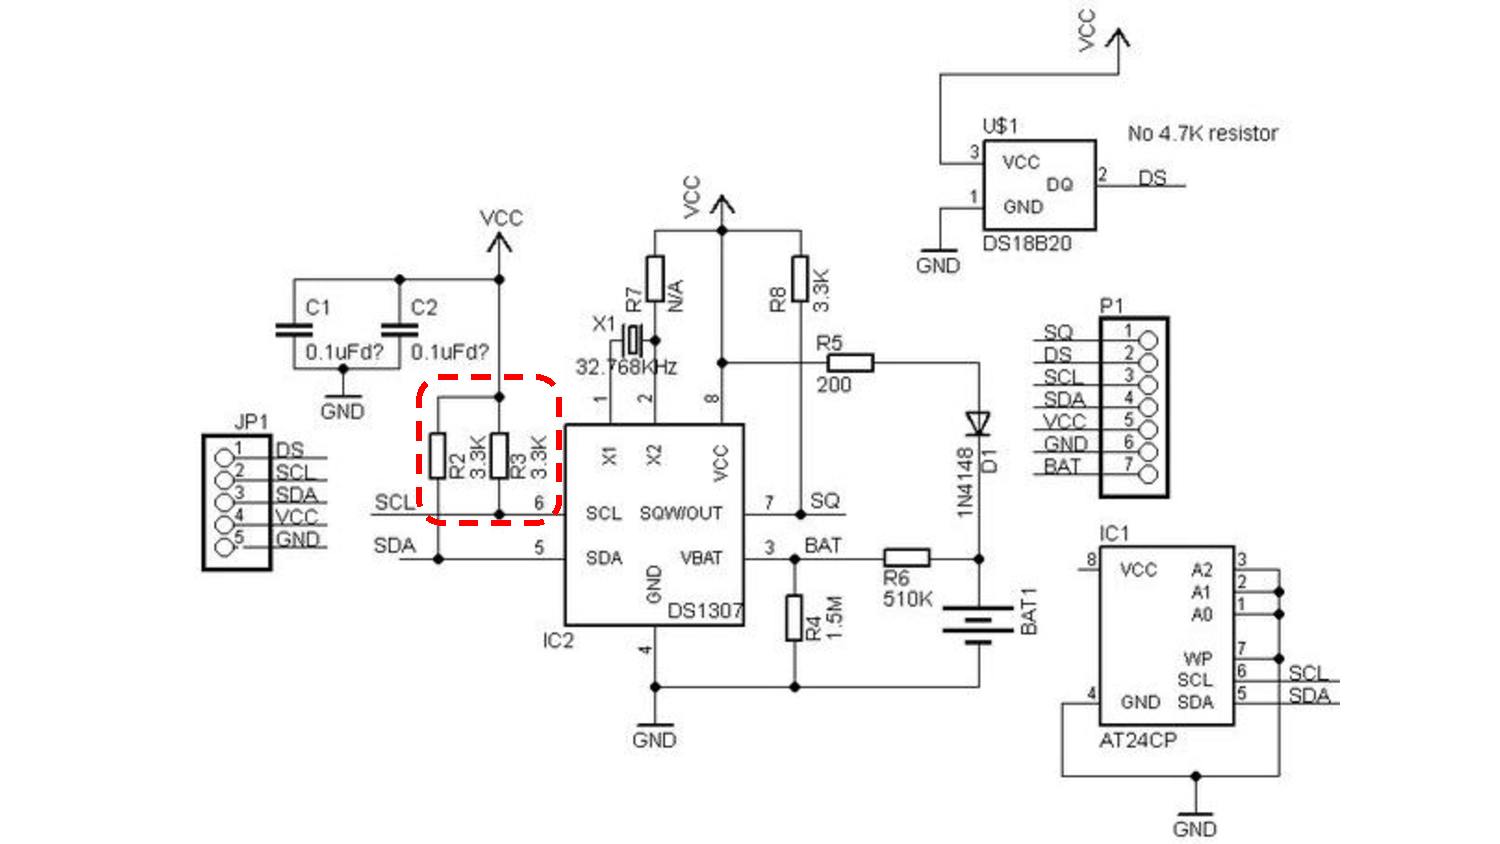
\includegraphics[width=0.9\linewidth,page=1]{ImagenesIngenieria de detalle/rtcTinySchematic}
	\caption{Esquemático RTC-Tiny.}
	\label{fig:RTCSchematic}
\end{figure}

Con este cambio se quita la referencia a $5 \ V$ del bus en el módulo. Por lo que la lógica queda en el rango de $3.3 \ V$ a $5 \ V$. Cabe destacar que utilizar los niveles lógicos de $3.3 \ V$ son compatibles con el integrado $DS1307$




\Subsubsection{Interfaz gráfica de usuario}
Para el desarrollo de la GUI, se valió del uso de \textbf{Node-Red}, software que permite el desarrollo de servicios online. Node-Red, mediante un sistema de nodos y sumado a la programación en JavaScript, permite generar una página web en una red local, lo cual cumple la función de interfaz con el usuario.

El sistema de edición y desarrollo de la GUI puede ser accedido a través de un navegador, de la misma manera que la interfaz del usuario. Para evitar que el usuario o alguna persona no deseada acceda a esta sección, se emplea un link privado, el cual es confidencial y no es publicado. También se vale de un sistema de autenticación que emplea la interfaz gráfica, creando un usuario de administrador.
\begin{figure}[H]
	\centering
	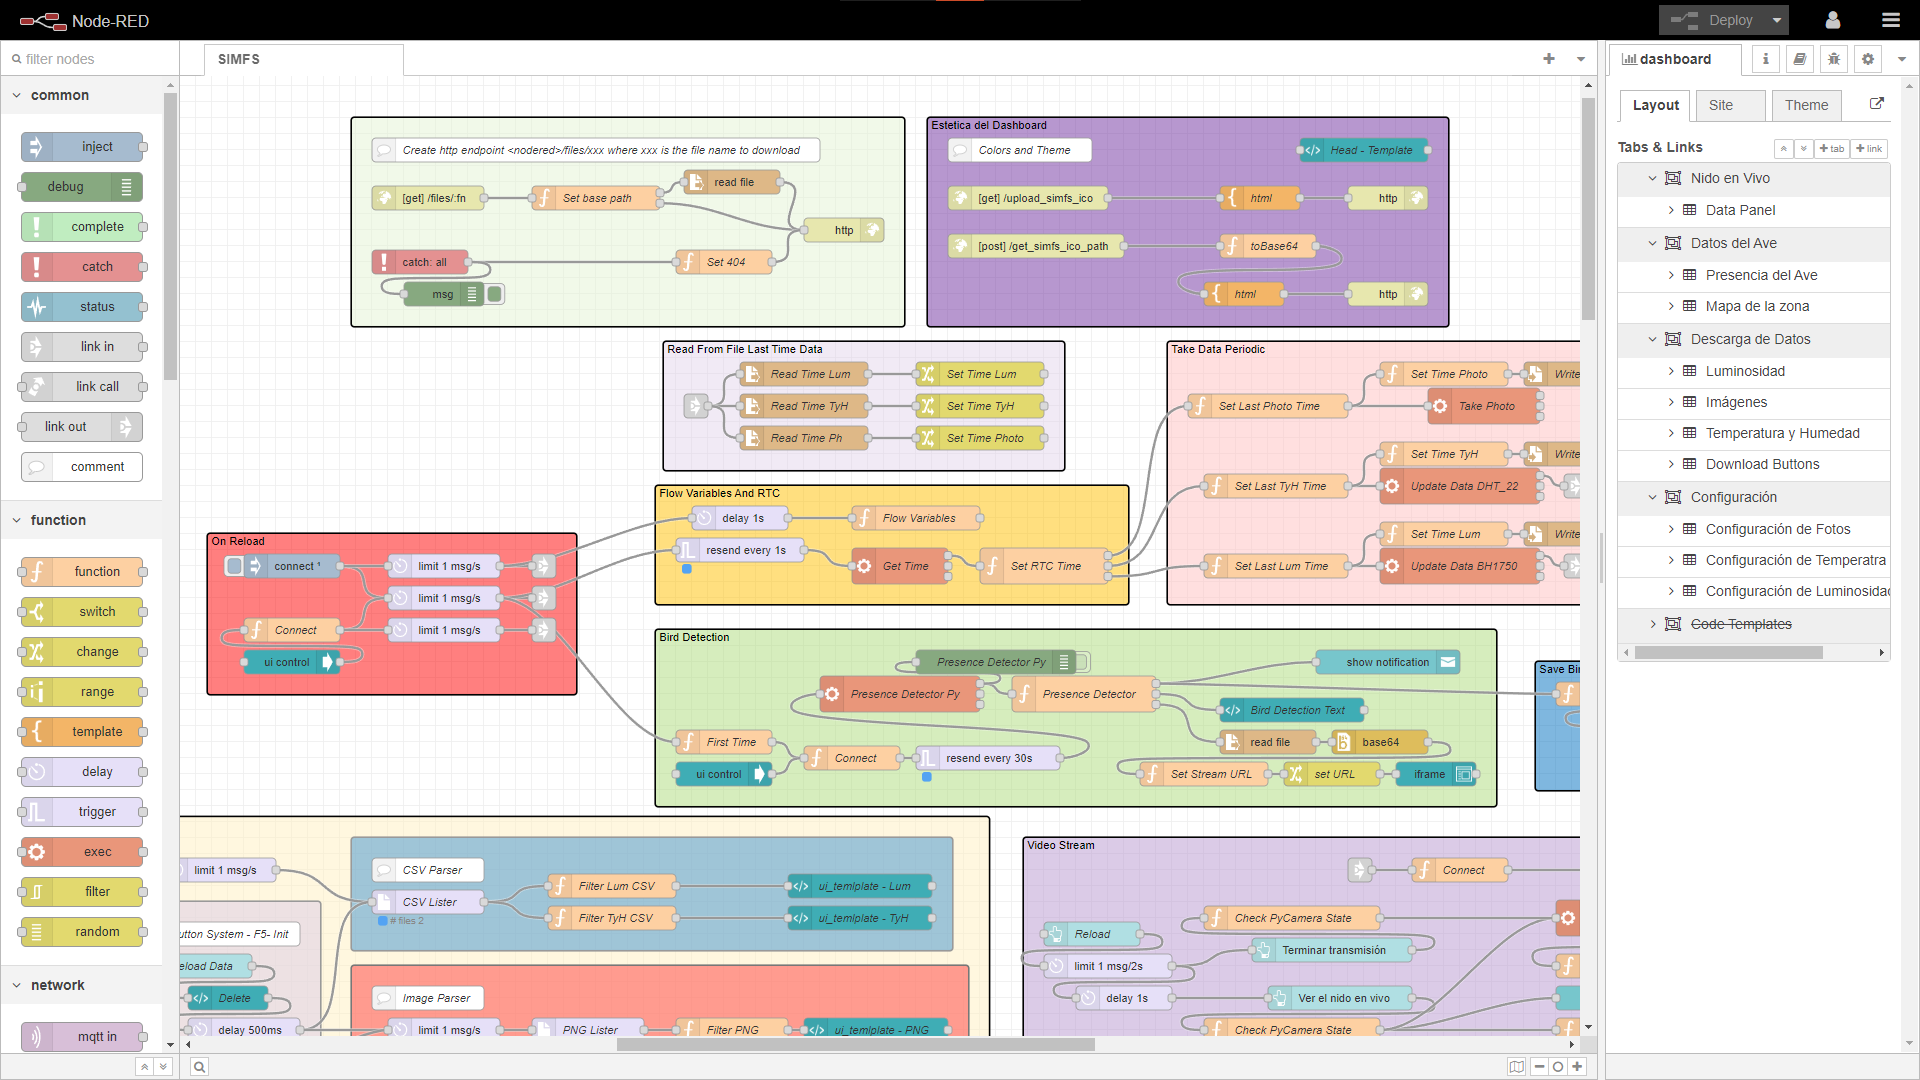
\includegraphics[width=0.9\linewidth]{ImagenesIngenieria de Detalle/Node-Red-Flow}
	\label{fig:node_red_flow}
	\caption{Flujo de nodos del servidor.}
\end{figure}

Dado que este servidor se encuentra corriendo en la R-Pi, al conectarse a la red de esta, se puede acceder a la página mencionada, donde se brindaran varias funcionalidades adicionales a las descargas básicas de los datos requeridos.

La interfaz gráfica a la cual el usuario tiene acceso posee distintas pestañas, donde cada una brinda un parámetro diferente. En la primer pestaña es posible ver las mediciones realizadas de luminosidad, temperatura y humedad en tiempo real. Además como el sistema detecta la presencia del ave, se muestra si este se encuentra dentro del nido o no. Por último se brinda al usuario la posibilidad de ver la una trasmisión en tiempo real del nido por dentro.
\begin{figure}[H]
\centering
    	\minipage{0.49\textwidth}
        	\centering
        	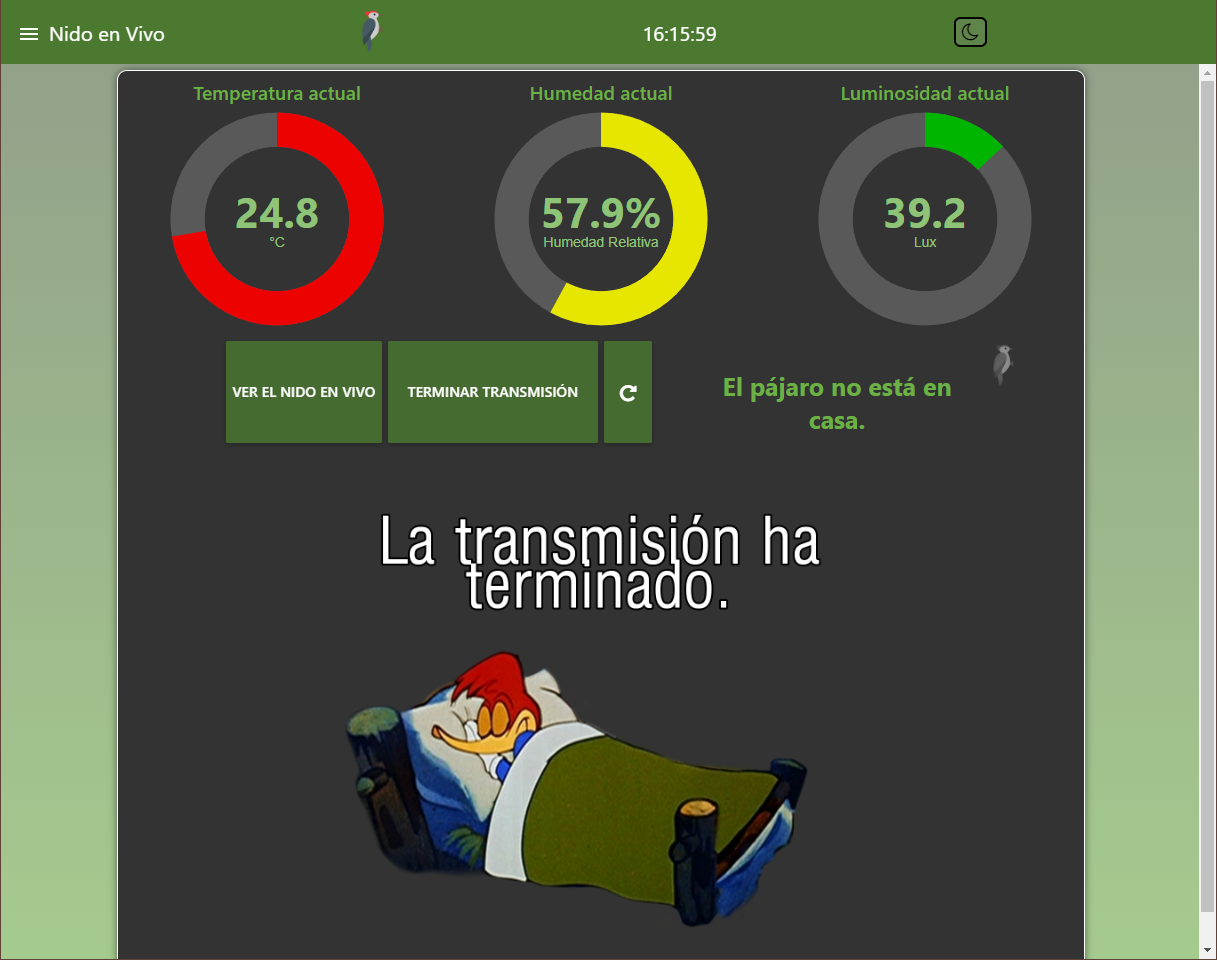
\includegraphics[width=\linewidth]{ImagenesIngenieria de Detalle/Node-Red-Live-Dark}		
			\caption{Interfaz con usuario versión oscura.}
			\label{fig:front_end_dark}
        \endminipage\hfill
        \minipage{0.49\textwidth}
        	\centering
        	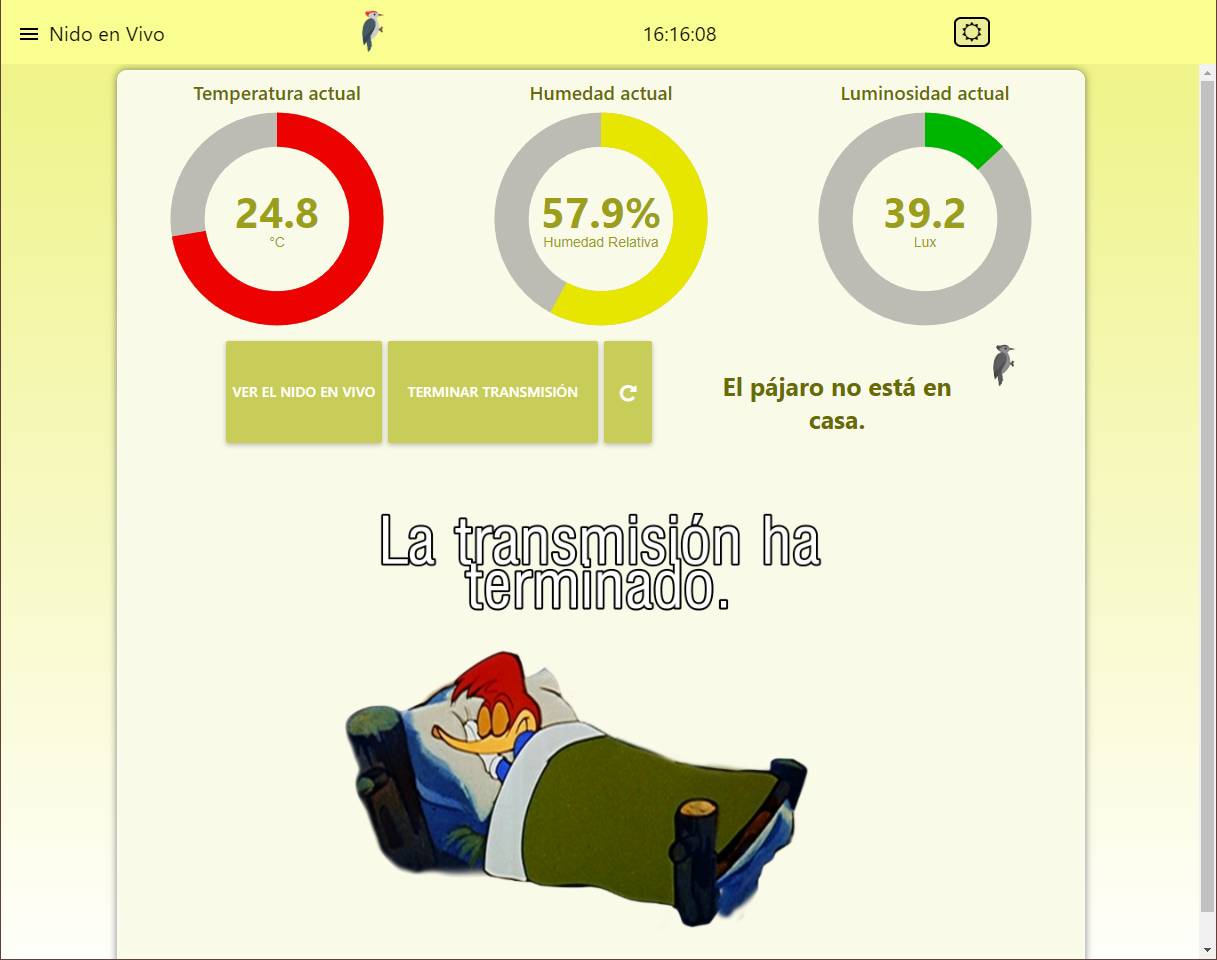
\includegraphics[width=\linewidth]{ImagenesIngenieria de Detalle/Node-Red-Live-Light}				\caption{Interfaz con usuario versión clara.}
			\label{fig:front_end_light}
        \endminipage
	\caption{Página del servidor a la cual accede el usuario.}
	\label{fig:node_red_live}
\end{figure}

En la segunda pestaña, es posible ver datos propios del ave, referidos a su posición. El primero muestra en un gráfico si el ave se ha encontrado dentro o fuera del nido durante un lapso de 24 horas, siendo posible seleccionar el día del cual se quiere ver los datos. Las zonas verdes denotan su estadía en el nido, mientras que las rijas su ausencia. Se muestra también cuanto tiempo duró cada intervalo. El segundo gráfico muestra el recorrido que ha realizado el ave en el entorno del nido en tiempo real.
\begin{figure}[H]
	\centering
    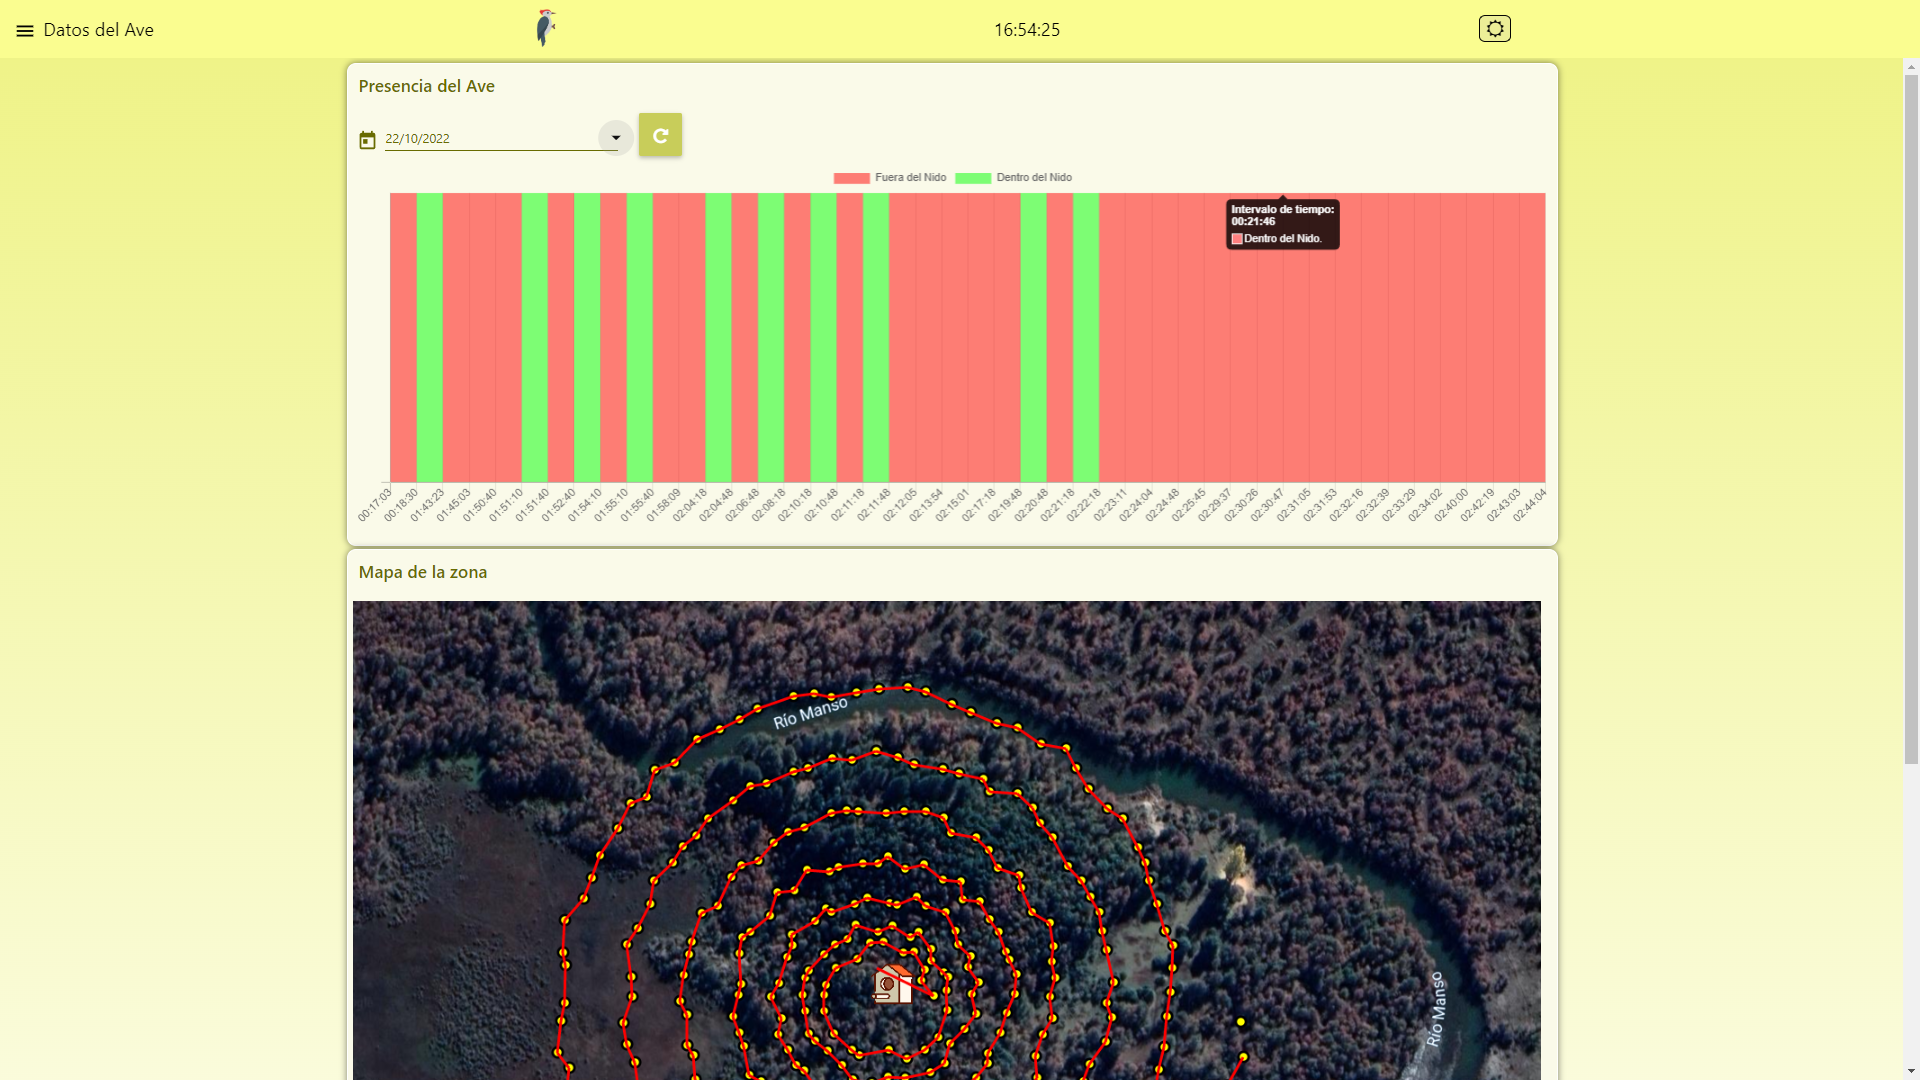
\includegraphics[width=0.7\linewidth]{ImagenesIngenieria de Detalle/Node-Red-Bird-Data}	
	\caption{Datos de presencia y posición del ave.}
	\label{fig:node_red_bird}
\end{figure}

La tercer pestaña es la más importante en cuanto a los requisitos del proyecto. En esta se presentan links de descarga para los datos obtenidos del nido y aquellos provistos por la unidad del pájaro. El usuario puede seleccionar el intervalo de tiempo en el cual desea obtener los datos.

Es posible descargar archivos del formato \quotes{csv} para los datos de luminosidad, temperatura y humedad, \quotes{png} si se desea descargar imágenes de forma individual o \quotes{zip} para el todo el conjunto de fotos mostradas.
\begin{figure}[H]
	\centering
    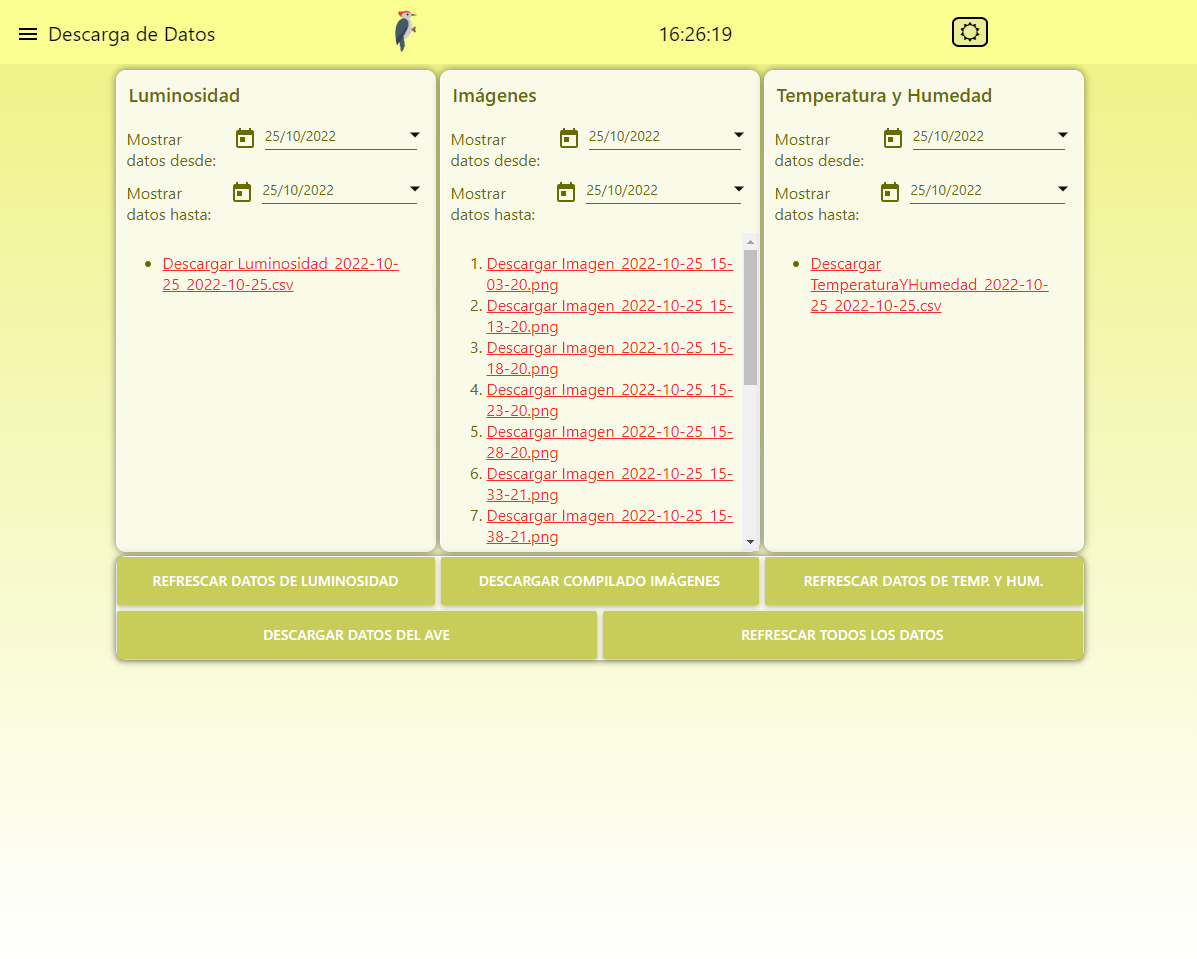
\includegraphics[width=0.7\linewidth]{ImagenesIngenieria de Detalle/Node-Red-Download}	
	\caption{Descarga de datos almacenados.}
	\label{fig:node_red_download}
\end{figure}

La cuarta y última pestaña le brinda al usuario cierto margen de configuración de la toma de datos. Estas opciones le permiten modificar el intervalo de cada medición, es decir cada cuanto tiempo se desea tomar una medición de las variables de interés o cada cuanto se desea tomar una foto.
\begin{figure}[H]
	\centering
    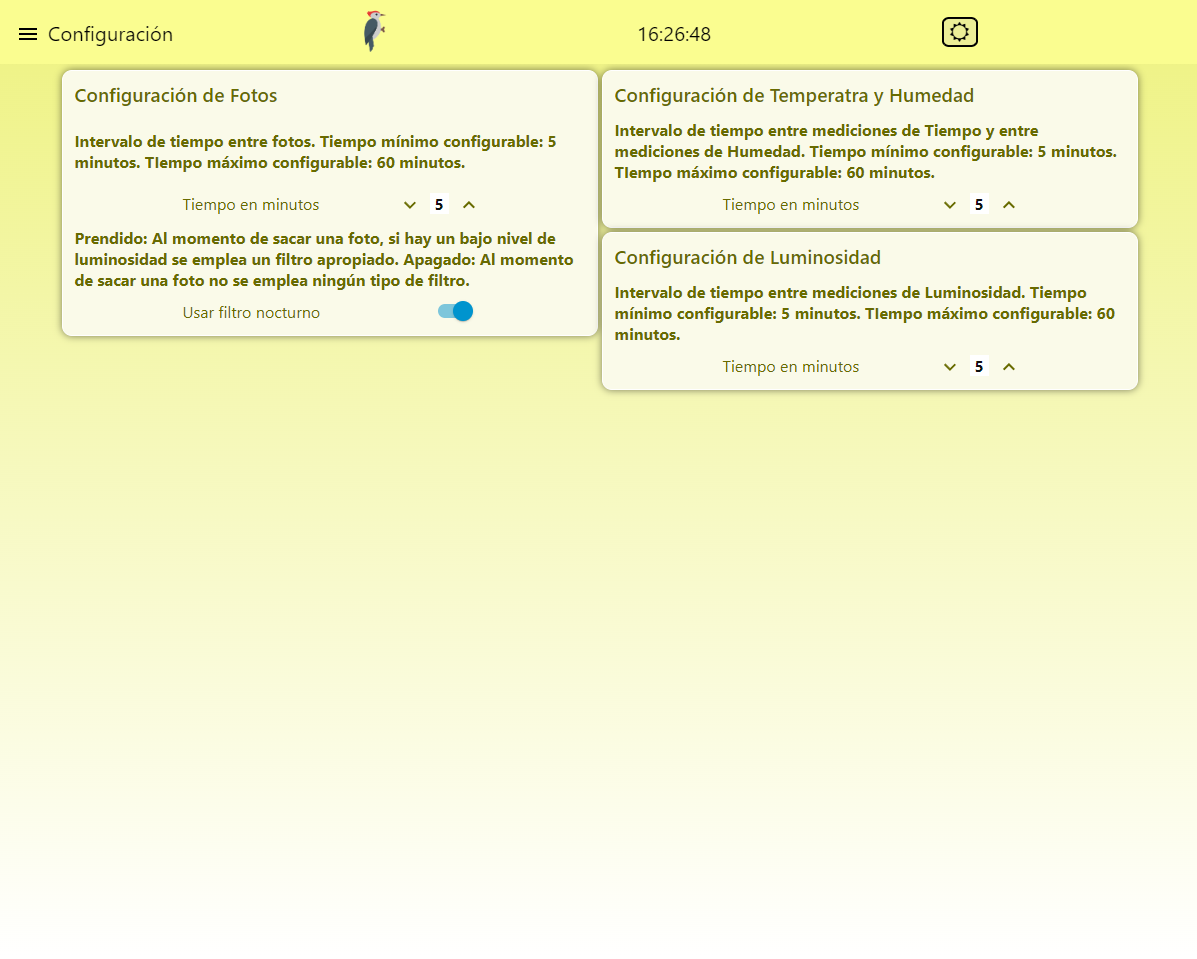
\includegraphics[width=0.7\linewidth]{ImagenesIngenieria de Detalle/Node-Red-Bird-Config}	
	\caption{Configuración de la interfaz gráfica.}
	\label{fig:node_red_config}
\end{figure}

También es posible determinar si se desea o no emplear un filtro en la cámara al momento tomar fotos, considerando el nivel luminosidad. En caso de que dicha variable posea un valor bajo se emplea el filtro mejorando así la luminosidad de la foto.
\begin{figure}[H]
\centering
    	\minipage{0.49\textwidth}
        	\centering
        	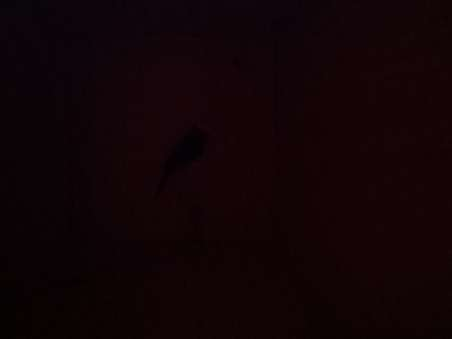
\includegraphics[width=\linewidth]{ImagenesIngenieria de Detalle/ImagenDevSF_2}		
			\caption{Foto tomada sin filtro de luminosidad.}
			\label{fig:foto_camara_sf}
        \endminipage\hfill
        \minipage{0.49\textwidth}
        	\centering
        	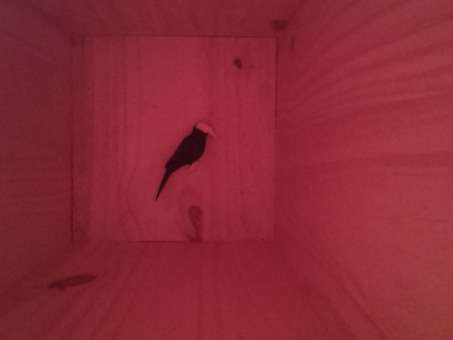
\includegraphics[width=\linewidth]{ImagenesIngenieria de Detalle/ImagenDevCF_2}					\caption{Foto tomada con filtro de luminosidad.}
			\label{fig:foto_camara_cf}
        \endminipage
	\caption{Comparación entre el uso del filtro de luminosidad.}
	\label{fig:foto_camara_filtro}
\end{figure}

Cabe destacar que de la misma forma que se considera un usuario de administrador, la GUI cuenta con una cuenta con contraseña para brindarle acceso al usuario y así evitar el uso de cualquier persona que consiga conexión a la red.

%\end{document}
